\documentclass[openany]{book}
\usepackage{ln}

\title{CSM EECS 20N Lecture Notes}
\author{Authored by Dun-Ming Huang, SID: 303******2}
\pgfplotsset{compat=1.18}
\setcounter{chapter}{0}

\begin{document}
\maketitle
\setcounter{tocdepth}{1}
\section{Preface}
Preface will be written later.

\tableofcontents
%\begin{comment}
\part{Linear Algebra is A Really Near Algebruh}
\chapter{The Fundamentals of Linear Algebra}
Hello
\newpage
\chapter{Arithmetics of Vectors and Matrices}
Hello

\section{Addition and Subtraction}
Hello

\section{Matrix Multiplication}
Hello

\section{Inverse Matrices}
Hello

\section{Determinants}
Hello

\newpage
\chapter{Gaussian Elimination}
Hello

\section{Linear Systems of Equations}
Hello

\section{Gaussian Elimination}
Hello

\section{Failure of Gaussian Elimination}
Hello

\newpage
\chapter{Linear Dependence}
Hello

\section{Linear Independence and Linear Dependence}
Hello

\section{Geometric Interpretation}
Hello

\section{Rank}
Hello

\newpage
\chapter{Vector Spaces}
Hello

\section{Definition of Vector Space}
Hello

\section{Subspaces}
Hello

\section{Columnspaces (Span)}
Hello

\section{Nullspaces (Kernel)}
Hello

\newpage
\chapter{Eigen Show You The World: Eigenvalues, Eigenvectors, and Eigenpain}
Hello % write about fixed point

\section{Eigenvalues}
Hello

\section{Eigenvectors}
Hello

\section{Eigenspaces}
Hello

\newpage
\chapter{Eigenspaces and Change of Basis}
Hello
\newpage
\chapter{Inner Products and Norms, Orthogonality}
Hello

\section{Inner Products of Vectors}
Hello

\section{Inner Product of Matrices}
Hello

\section{Norms of Vectors}

\subsection{Definition of Vector Norms}
In prior courses, we have recognized the following symbol:
\begin{ln-symbol}{Euclidean Norm}{}
    The Euclidiean Norm, otherwise known as a \textbf{2-Norm}, is a mathematical quantity for some vector $\vec{x}$:
    \[
        {\lVert \vec{x} \rVert}_2 = \sqrt{\sum_i x_i^2}
    \]
    which measures the Euclidean distance (Pythagorean Theorem's results) between the starting and terminal point of a vector.
\end{ln-symbol}
While the Euclidean Norm is an extremely common norm, there exist more norms to vectors. \\
Particularly, \textbf{norms} are functions that satisfy the following properties:
\begin{ln-define}{Norm}{}
    A norm is a function $f: \mathcal{X} \rightarrow \R$ such that:
    \begin{bindenum}
        \item[1.] Non-negativeness: $\forall \vec{x} \in \mathcal{X}, \lVert \vec{x} \rVert \geq 0$, and $\lVert \vec{x} \rVert = 0 \iff \vec{x} = \vec{0}$
        \item[2.] Triangle Inequality: $\forall \vec{x}, \vec{y} \in \mathcal{X}, \lVert \vec{x} + \vec{y} \rVert \leq \lVert \vec{x} \rVert + \lVert \vec{y} \rVert$
        \item[3.] Scalar Multiplication: $\forall \alpha \in \R, \vec{x} \in \mathcal{X}, \lVert \alpha \vec{x} \rVert = \alpha \lVert \vec{x} \rVert$
    \end{bindenum}
\end{ln-define}

It is noteworthy to mention that, almost every norm demonstrates one property of the vector.
For the diversity of characteristics that a vector may have, there certainly exists a diversity of norms for vectors.
For example, a general family of norms that satisfy the above properties would be the \textbf{LP-norms}:
\begin{ln-define}{LP-Norms}{}
    LP-Norms are norm functions defined as:
    \[
        {\lVert \vec{x} \rVert}_p = {\bigg( \sum_{i = 1}^n |x_i|^p \bigg)}^{\frac{1}{p}}
    \]
    for some natural number $p$. \\
\end{ln-define}
Particularly, the Euclidean Norm, otherwise known as the \textit{2-norm} is LP-norm with $p = 2$. \\
Meanwhile, the $1$-norm and $\infty$-norm are defined as follows:
\begin{align*}
    {\lVert \vec{x} \rVert}_1 &= \sum_{i = 1}^n |x_i| \\
    {\lVert \vec{x} \rVert}_\infty &= \max_{i = 1, \dots, n} |x_i|
\end{align*}
where, the $1$-norm of a vector can be stated as the Manhattan distance (Taxicab geometry) of between that vector's starting and terminal point.

\subsection{Cauchy-Schwartz Inequality}
This inequality was active in EECS 16A!
\begin{ln-define}{Cauchy-Schwartz Inequality}{}
    The inequality is phrased as:
    \[
        |\vec{x}^T \vec{y}| \leq {\lVert \vec{x} \rVert}_2 {\lVert \vec{y} \rVert}_2
    \]
    And using the property,
    \[\forall x \in \R, |\cos(x)| \leq 1\]
    \tcblower
    This inequality originates from the following algebraic work:
    \begin{align*}
        |\langle \vec{x}, \vec{y} \rangle| &= |\vec{x}^T \vec{y}| = |\vec{y}^T \vec{x}| \\
        &= |{\lVert \vec{x} \rVert}_2 {\lVert \vec{y} \rVert}_2 \cos(\theta_{\vec{x}, \vec{y}})|
        \leq |{\lVert \vec{x} \rVert}_2 {\lVert \vec{y} \rVert}_2|
    \end{align*}
\end{ln-define}

We observe that the above derivation holds statement on equivalence between inner product and product of magnitudes, cosine. \\
That is justified by the mechanics along which we find the projection of $\vec{y}$ onto $\vec{x}$:
\[
    \proj{\vec{x}}{\vec{y}} = \vec{x} \frac{\vec{x}^T\vec{y}}{{\lVert \vec{x} \rVert}_2^2}
\]
where, since the projection is a multiple of $\vec{x}$ such that $\proj{\vec{x}}{\vec{y}} = t\vec{x}$, we also recognize that,
\[
    \cos(\theta_{\vec{x}, \vec{y}}) = \frac{{\lVert t\vec{x} \rVert}_2}{{\lVert \vec{y} \rVert}_2}
\]
Upon matching the two equations, I acquire:
\begin{align*}
    t = \cos(\theta_{\vec{x}, \vec{y}}) \frac{\pnorm{\vec{y}}{2}}{\pnorm{\vec{x}}{2}} &= \frac{\vec{x}^T\vec{y}}{\pnorm[2]{\vec{x}}{2}} \\
    |{\lVert \vec{x} \rVert}_2 {\lVert \vec{y} \rVert}_2| &= \langle \vec{x}, \vec{y} \rangle
\end{align*}

In fact, we find that the Cauchy-Schwartz is a general case of this inequality:
\begin{ln-define}{Holder's Inequality}{}
    Provided the quantities
    \[\vec{x}, \vec{y} \in \R^n, \text{and some } p, q \geq 1 \text{ s.t. } \frac{1}{p} + \frac{1}{q} = 1\]
    Then, 
    \[|\vec{x}^T \vec{y}| \leq {\lVert \vec{x} \rVert}_p{\lVert \vec{y} \rVert}_p\]
\end{ln-define}

\subsection{Application of Cauchy-Schwarz Inequality: Norm Ball}
From this concept, let us consider the concept of \textit{``norm ball''}: the geographical object containing all vectors such that their lp-norm is $1$.

\begin{bindenum}
    \item For a $2$-norm, for example, the norm ball looks like a unit circle (containing all 2D vectors with length $1$, hence a circle of radius $1$).
    \item For a $1$-norm, similar logic guides us to a diagonally placed circle (rotated $45^\circ$) centered at the origin with side lengths $2$.
    \item For the $\infty$-norm, has a norm ball of a square centered at origin with side length $2$. This embeds the unit ball from $2$-norm, which embeds the unit ball from $1$-norm.
\end{bindenum}
The last bullet point hints that the area of norm ball is larger for any increase in $p$ such that it embeds the prior norm balls.
\par
Now, let us attempt to solve for some optimization regarding a norm ball:
\[\max_{\pnorm{\vec{x}}{p} \leq 1} \vec{x}^T \vec{y}\]

\underline{\textbf{p = 2}}:
\begin{quote}
    The solution would be, by the Cauchy Schwartz's implication,
    \[\vec{x}^* = \frac{\vec{y}}{\lVert \vec{y} \rVert}_2\]
\end{quote}
\underline{\textbf{p = 1}}:
\begin{quote}
    The expression of dot product is equivalently
    \[x_1 y_1 + \cdots + x_n y_n\]
    Where the constraint is
    \[|x_1| + \cdots + |x_n| \leq 1\]
    For each value the components of $\vec{x}$, which is finite and upper bounded by $1$, we should allocate maximum contribution to the maximum element of $\vec{y}$ to maximize this dot product (a weighted sum of $\vec{y}$'s component, essentially). \\
    Therefore, let $i$ be the index at which $\vec{y}$ has the component of largest absolute value,
    \begin{quote}
        There is an achievable solution for $\vec{x}^*$, being the unit vector $\vec{e}_i$ multiplied by $sgn(y_i)$, so to counter for cases where $\vec{y}$ is negative.
    \end{quote}
    \par
    In turn, we see that
    \[\vec{x}^T \vec{y} = \max_i |y_i| = {\lVert \vec{y} \rVert}_\infty\]
    Meanwhile, let us use the Holder's Inequality to achieve a more rigorous proof. Holder's Inequality states that,
    \[
        |\vec{x}^T \vec{y}| \leq {\lVert \vec{x} \rVert}_1 {\lVert \vec{y} \rVert}_\infty = \max_i |y_i|
    \]
    \begin{quote}
        The Holder's Inequality expresses \textbf{an upper bound}, and the formulation in above section shows \textbf{achievability of upper bound}.
    \end{quote}
    \textbf{\textit{Alternative proof of p = 1 via Triangle Inequality}}: \\
    Via the triangle inequality, we acquire:
    \begin{align*}
        |\vec{x}^T \vec{y}| &= |\sum_i x_i y_i| \\
        &\underset{Triangle\ Inequality}{\leq} \sum_i |x_i y_i| \\
        &= \sum_i |x_i||y_i| \\
        &\leq \sum_i |x_i| \max_i |y_i| = \max_i |y_i| = {\lVert \vec{x} \rVert}_\infty
    \end{align*}
    We see the expression $|\vec{x}^T \vec{y}|$ has an \textbf{achievable upper bound}, assembling all necessary aspects of deriving the solution for the optimization problem.
\end{quote}
\underline{\textbf{p = $\infty$}}:
\begin{quote}
    We can find upper bound of the expressionvia Holder's Inequality,
    \[
        |\vec{x}^T \vec{y}| \leq {\lVert \vec{x} \rVert}_\infty {\lVert \vec{y} \rVert}_1 \leq \sum_i |y_i|
    \]
    The infinity norm of $\vec{x}$ shows the constraint that:
    \[
        \max_i |x_i| = 1
    \]
    and we may simply compute:
    \[
        x_i = sgn(y_i)
    \]
    to find and certify the achievability of this upper bound.
\end{quote}

\section{Norms of Matrices}
Hello

\newpage
\chapter{Least Squares Algorithm: Where Machine Learning Starts}
Hello

\section{Overdetermined Systems}
Hello

\section{Estimation of Solutions for Overdetermined Systems}
Hello

\section{Summary of Least Squares Algorithm}
Hello


\part{New Mathematical Prerequisites}
\chapter{An Integral Review for Integration}
Hello
\newpage
\chapter{Set!}
Hello
\newpage

\chapter{Propositional Logic}

\section{Definition of Proposition}
To speak the language of mathematics, we must familiarize ourselves with objects of the mathematical language. One fundamental block of this mathematical language is a \textbf{proposition}.
\begin{ln-define}{Proposition}{}
    A proposition is a logical statement that is either true or false. \\
    In other words, it is a mathematical statement that could be correct, but also could be incorrect.
\end{ln-define}
Propositions need to be either true or false, which means it cannot be statements that can yield some ambiguous result. \\
And because they usually are not known to be true or false, we often need to prove propositions in discrete mathematics.
\begin{ln-think}{What should a proposition be like?}{}
    Which of the following qualifies as a proposition?
    \begin{enumerate}
        \item[(a)] $\sqrt{3}$ is rational.
        \item[(b)] 2 + 2
        \item[(c)] I often never give up or let down
    \end{enumerate}
    \tcblower
    Option (a) is a statement that has to either hold true or false, because this value $\sqrt{3}$ is either rational or irrational. \\
    Option (b) is a mathematical expression, and there is no true or false aspect to it. It is not a proposition. \\
    Last but not least, option (c) is just a statement, because the word ``often`` is not properly defined. If propositions are supposed to clearly hold true or false, it should not contain blurrily defined words. \\
    The answer, therefore, is option (a).
\end{ln-think}

\section{Logical Operations of Proposition}
There are approximately four methods of using preexistent propositions to make new propositions, and we do so to produce complicated propositions from simpler subparts. \\
These four ways being:
\begin{bindenum}
    \item \textbf{Conjunction}: $P \land Q$, works similarly as the boolean ``and``.
    \item \textbf{Disjunction}: $P \lor Q$, works similarly as the boolean ``or``.
    \item \textbf{Negation}: $\neg P$, works similarly as the boolean ``not``.
    \item \textbf{Implies}: $P \implies Q$, which states a familiar phrase of ``if P, then Q``. Here, the proposition $P$ is called a hypothesis, and $Q$ a conclusion.
\end{bindenum}
To demonstrate the behaviors of these operations, we may use a \textbf{truth table}. A truth table example for the operation ``Conjunction`` is attached below:
\begin{ln-fig}{Truth Table for Conjunction}{}
    A truth table is a table that points out the result of an operation on statements $P$ and $Q$, for a set of given boolean values that $P$ and $Q$ each result in.
    \begin{center}
        \begin{tabular}{c c||c}
            $P$ & $Q$ & $P \land Q$ \\
            \hline
            T & T & T \\
            \hline
            T & F & F \\
            \hline
            F & T & F \\
            \hline
            F & F & F
        \end{tabular}
    \end{center}
\end{ln-fig}
Now we may discuss some other properties of propositions. \\
First of all, there is a fundamental principle called \textbf{Law of the Excluded Middle}, which states what is as follows:
\begin{ln-axiom}{Law of Excluded Middle}{}
    For any proposition $P$, $P \lor \neg P$ always holds true, because $P$ is either true or false (not true).
\end{ln-axiom}
Here, propositions like $P \lor \neg P$ that always hold true are called \textbf{tautologies}. \\
Meanwhile, propositions that are always false, such as $P \land \neg P$ (which cannot be true, since $P$ is either true or false), are called \textbf{contradictions}. \\
Implications also have interesting truth table properties:
\begin{ln-fig}{Truth Table for Implication}{}
    A truth table for implications is as follows:
    \begin{center}
        \begin{tabular}{c c||c c}
            $P$ & $Q$ & $P \implies Q$ & $\neg P \lor Q$ \\
            \hline
            T & T & T & T \\
            \hline
            T & F & F & F\\
            \hline
            F & T & T & T\\
            \hline
            F & F & T & T
        \end{tabular}
    \end{center}
    While this provides that the implication is only false when $P$ is true and $Q$ is false, this also provides a not so intuitive insight: An implication is trivially true when the hypothesis is false. \\
    This situation is known as \textbf{``vacuously true''}. \\
    The reason why this insight seems to hold is because while we cannot confirm the conclusion is false when the hypothesis is false, this is also the nature of how if-then statements are expected to be defined. \\

    Indicated via the above truth table, as $P \implies Q$ and $\not P \lor Q$ have the exact same boolean behavior on truth table, they are logically equivalent. This means they are statements that perform the logical behavior and meaning.
\end{ln-fig}
Interestingly, there are also various ways to pronounce implications, such as ``if P, then Q``, as well as ``Q if P``, and many more. \\
Sometimes we also come across words that seem to connect two propositions in a tighter implication, such as ``iff``. \\
An \textbf{iff} relationship is also standardly pronounced as \textbf{if and only if}, which is mathematically expressed as $P \iff Q$. This ``iff`` holds if both $P \implies Q$ and $Q \implies P$ are true. Consequentially, and as encountered in previous coursework, such as EECS 16A, the proof of an ``iff`` statement is at its nature the proof of two smaller statements.

\section{Implications from Implications}
For an implication $P \implies Q$, we may define two other implications out of it:
\begin{bindenum}
    \item \textbf{Contrapositive}: $\neg Q \implies \neg P$, which is logically equivalent to $P \implies Q$. At its implication: if a statement $P$'s contrapositive is true, so should the statement $P$ per se.
    \item \textbf{Converse}: $Q \implies P$, which does not always hold true. In some cases, converse statements can hold true, but usually accompanies some extra conditions. Some examples can be observed in the contents of MATH 53.
\end{bindenum}

When two propositions are logically equivalent, we may mathematically denote it with the $\equiv$ symbol. \\
An example of usage would be stating an implication the logical equivalent of its contrapositive, in the forms:
\[(P \implies Q) \equiv (\neg Q \implies \neg P)\]
An application of this is a new approach of performing proofs. To prove a prompt that states a theorem as an implication $P \implies Q$, by proving its contrapositive, which is in some cases easier than proving the prompt directly, we can manage to indirectly prove the prompt. \\
This application will be introduced in the next chapter as ``proof by contrapositive''.

\section{Quantifiers}

\subsection{Use of Quantifiers}
In the previous chapter, we introduced the usage of quantifiers as an abbreviation and selector of elements in sets to which a condition holds, in the format of:
\[\text{<quantifier selecting clause> <second clause containing condition to hold for selected values>}\]
The second clause is effectively a proposition, while the entire sentence containing the first and second clause is also effectively a proposition.

There is a more sophisticated way to express the first clauses of these forms of propositions. \\
The first clause has a quantifier, and throughout a ``universe'' we are working with (abstractly, a wide variety of mathematical objects following some conventions), the statement is quantified (holding true) for a selected range of objects in this universe. \\
So syntactically, the quantifier serves to involve this range of quantification for our proposition.

Let me expound on this abstraction of ``universe'' further. Say we attempt to qualify a proposition on all natural numbers, such as:
\[
    \forall x \in \N, x \in \Q
\]
Then, the total set of objects I'm working through is the set of all natural numbers, and is therefore the \textbf{``universe'': a collection of all objects to be qualified in this proposition}.
In that sense, universe is a set.

In a finite universe, there is also another way of conceptualizing the quantifiers we know:
\begin{ln-think}{Propositional Logic in Quantifiers}{}
    Let us work with a universe $\U = {U_1, \dots, U_n}$, where $n$ is some finite natural number and elements of this universe are some mathematical object. \\
    Then:
    \begin{bindenum}
        \item \textbf{Universal Quantifiers}: $(\forall x \in \U (P(x))) \equiv (P(U_1) \land \dots \land P(U_n))$
        \item \textbf{Existential Quantifiers}: $(\exists x \in \U (P(x))) \equiv (P(U_1) \lor \dots \lor P(U_n))$
    \end{bindenum}
\end{ln-think}
To express more complicated propositions, we must expand beyond the previous first-clause-second-clause format for propositions. This is especially when we are selecting two ranges of values to describe a multi-variable proposition with.
\begin{ln-think}{How to read complicated propositions?}{}
    Say we are dealing with the proposition:
    \[(\forall x \in \Z)(\exists y \in Z)(x < y)\]
    Here, I can observe two quantifying clauses and the last clause that stands for a proposition. In fact, propositions involving quantifiers will always have the last clause as a proposition, due to the syntactical limits and customs of mathematical language. \\
    Now let us try translating each clause into the English language:
    \begin{enumerate}
        \item $\forall x \in \Z$: For all objects $x$ that belongs to $\Z$, the set of all integers.
        \item $\exists y \in \Z$: There exists an object $y$ that belongs to $\Z$, the set of all integers.
        \item $x < y$: Object $x$ is smaller than $y$.
    \end{enumerate}
    Piecing the clauses together: For all objects $x$ that belongs to $\Z$, the set of all integers, there exists an object $y$ that belongs to $\Z$ such that $x$ is smaller than $y$. \\
    This proposition, in fact, holds true, since we can always find a larger integer. \\
    However, the proposition with a reversed order for quantifier clauses:
    \[(\exists y \in Z)(\forall x \in \Z)(x < y)\]
    has to hold False. \\

    With the above translating process, this statement states that: there is an object $y$ that belongs to $\Z$, the set of all integers, such that for all objects $x$ that belongs to $\Z$ such that $x$ is smaller than $y$. \\
    In other words, it assumes the existence of one largest integer, which does not exist!
\end{ln-think}

Then, let us look at an example from the Fall 2022 Midterm 1:
\begin{ln-example}{Reading Complicated Quantifier Statements}{}
    Which logical expression(s) below correspond to the predicate that $p$ is prime? \\
    \begin{bindenum}
        \item[a.] $(\forall b \in \N) \big( (b \leq 1) \lor \neg(\exists a \in \N)(a \neq 0 \land ab \neq p) \big)$
        \item[b.] $\neg\big( (\exists a, b \in \N) ((a \geq 2) \land (a < p) \land (p = ab)) \big)$
    \end{bindenum}
    \tcblower
    For the expression (a), it states that:
    \begin{quote}
        For all natural numbers $b$, either $b \leq 1$ or there does not exist a natural number $a$ such that $a$ is nonzero and $ab \neq p$. \\
    \end{quote}
    Therefore, for any positive integer $b$ larger than $2$, there does not exist another positive integer $a$ such that $ab \neq p$. \\
    However, let's consider the possibility $p = 2$, which is prime, then for an integer $b = 2$, there exists $a = 1$ such that $ab = 2$. \\
    Therefore, the trueness of expression (a) does not indicate that $p$ is prime. \\

    Now, consider expression (b), which instead states that:
    \begin{quote}
        It is not such that there exists two natural numbers $a$, $b$ where simulatneously, $a \geq 2$, $a < p$, and $p = ab$.
    \end{quote}
    To simplify the above quote, there does not exist a pair of natural numbers such that when one of them is a natural number $2 \leq a < p$, the other number multiplied by this number is $p$. \\
    Since $a < p$, to achieve $ab = p$, it is impossible that $b = 1$. This successfully circumvents the limitation encountered in expression (a), qualifying expression (b) as the correct solution. This expression does successfully describe the definition of prime number $p$:
    \begin{quote}
        The only pair of natural number whose product is prime $p$ is $(1, p)$
    \end{quote}
    By demonstrating that there exist no pair of natural number whose product is $p$ if one of the element is exclusively between $1$ and $p$.
\end{ln-example}
This is an interesting discussion, as the question presented above has in fact been regraded!

\section{Reading and Negation}
\subsection{Meaning of Negation}
If a proposition $P$ is false, its negation is true. \\
This inspires another approach for proofs (proof by contradiction), which usually work for simpler prompts since their contradictions would only be simpler to prove, if provided that this method is optimal to begin with. \\
However, when $P$ appears to be a more complicated proposition involving other smaller propositions, we should look for some way to make our understanding of it more concise. \\
A logical law, called the \textbf{De Morgan's Laws}, facilitates us with such matter:
\begin{ln-axiom}{De Morgan's Law}{}
    The De Morgan's Law states the two following logical equivalences:
    \[\neg (P \land Q) \equiv (\neg P \lor \neg Q)\]
    \[\neg (P \lor Q) \equiv (\neg P \land \neg Q)\]
\end{ln-axiom}
In fact, negations of propositions involving quantifiers follow analogous laws, due to the similarity of universal quantifier with conjunction and existential quantifier with disjunction:
\begin{ln-axiom}{Extension of De Morgan's Law}{}
    Based on the similiarity of quantifiers with operations of propositions:
    \[\neg (\forall x P(x)) \equiv (\exists x \neg P(x))\]
    \[\neg (\exists x P(x)) \equiv (\forall x \neg P(x))\]
\end{ln-axiom}
These above equivalences can provide flexibility in coming mathematical proofs.

\subsection{Complex Examples of Negation}
Let us discuss the example attached on the lecture notes from Summer 2022.
\begin{center}
    \textbf{Prompt 1: Write a proposition that states, ``there are at least three distinct integers $x$ that satisfies $P(x)$.}
\end{center}
And the proposition our textbook provided was:
\[\exists x \exists y \exists z (x \neq y \neq z \land P(x) \land P(y) \land P(z))\]
\begin{ln-think}{Proposition for Prompt 1}{}
    Let us analyze this proposition via some translation:
    \begin{align*}
        &\exists x \exists y \exists z (x \neq y \land x \neq z \land y \neq z \land P(x) \land P(y) \land P(z)) \\
        &\rightarrow \text{``there exists a x, y, z'' such that} \\
        & \text{``x, y, z are not equal to each other, and all of $P(x), P(y), P(z)$ holds''.} \\
        &\rightarrow \text{``there exists at least one possible combination of three distinct integers''} \\
        & \text{such that ``all of $P(x), P(y), P(z)$ holds``.} \\
        &\rightarrow \text{there are at least three distinct integers $x$ that satisfies $P(x)$.}
    \end{align*}
\end{ln-think}
In the above translation process, we first analyzed each phrases independently. Then, having each clauses translated, we move on to combine them together semantically. \\
For example, the fact that the three integers $x$, $y$, $z$ are not equal to each other means they are distinct, and so we may summarize the quantifying clause from ``there exists a $\dots$'' into ``there exists at least one combination of three integers such that $\dots$''. \\
This helps us imply that, if there exists at least one combination, then there are at least three integers to satisfy $P(x)$. \\
This logic of inter-language and inter-context translation allows us to convert a proposition from its mathematical form to pure English text. It should be familiarized via practice and experience. \\
For purposes of practicing, let us analyze another proposition and attempt to translate it:
\[\exists x \exists y \exists z \forall d (P(d) \implies d = x \lor d = y \lor d = z)\]
And in the following portion, let us perform again the same procedure of directly translating the proposition from symbols to English, and then rephrase each English clause into more concise descriptions.
\begin{ln-think}{Explain this proposition for me, will you?}{}
    Translate the proposition to English: $\exists x \exists y \exists z \forall d (P(d) \implies d = x \lor d = y \lor d = z)$
    \tcblower
    This proposition first has a quantifying clause that states: ``there exists a $x$, $y$, and $z$ for all values $d$``, or that there exists a set of three numbers $x$, $y$ and $z$ for all values $d$. \\
    The last clause is an implication stating: ``if $P(d)$ holds true, then $d = x \lor d = y \lor d = z$''. That means $d$ is equal to either $x$, $y$, or $z$. So, there exists three numbers out of all possible values in the universe such that if $P(d)$ holds, then $d$ is one of the three numbers we observed before. \\
    Meanwhile, we are not provided that $x$, $y$, and $z$ are distinct values, so there are at most three values for $d$ such that $P(d)$ holds.\\
    Let us switch a perspective and view the contrapositive of the later clause and verify our previous interpretation. If $d$ is equal to neither of $x$, $y$, $z$, then $P(d)$ will not hold. \\
    Assuming they are distinct, this statement would provide that if $d$ is equal to neither of some (up to three) distinct numbers, $P(d)$ will not hold. \\
    Therefore, the proposition is stating ``\textbf{$P(d)$ holds for at most three distinct integers}''.
\end{ln-think}
Here is one demonstration about conjunctions. \\
By performing conjunction for the propositions above: that $P(d)$ holds for at least and at most 3 integers, we successfully create a new proposition that states ``$P(d)$ holds for exactly 3 integers``. \\
Mathematical propositions that come with limits, or quantifying clauses, for some other proposition are useful in helping us locate a range of values for which a condition holds. 

If we combine propositions that hold for same conditions but with different quantified limits, we managed to combine the limits together and form some tighter statement providing a proposition with tighter limitations.

\newpage
\chapter{Introduction to Signals}
Hello

\part{Introduction to Signals and Systems}
\chapter{Introduction to Systems}
Hello
\newpage
\chapter{Mathematical Definitions for Functions and Signals}
Hello
\newpage
\chapter{Mathematical Definitions for Signals and Systems}

\section{Defining Signals}
Because a signal is fundamentally a function, the conventions of defining a signal closely follow the conventions of defining a function.
For example, suppose we would like to define an audio signal as a function of time that returns the soundwave air pressure of some specific point, then we can simply define this function declaratively as:
\[
    \forall t \in {\rm Time}, s(t) = \sin(440 \times 2\pi t)
\]
which states that the air pressure of our sound signal is a sinusoidal function with respect to time.

On the other hand, we may also define our function imperatively when programming the signal, which would result in the portrayal of abbove function using code:
\begin{verbatim}
import numpy as np
signal = lambda t: np.sin(440 * 2 * np.pi * t)
\end{verbatim}
You will be frequently using imperative definitions in lab assignments, and declarative definitions when working with the mathematical representation of signal in homework assignments or exams.

\section{Defining Systems}
\subsection{A Review of Systems}
Remember that we define systems as functions that map an input signal space (a space of all possible input signals) onto an output signal space.
Therefore, systems are functions whose domains and ranges can be expressed in: $S: [D \rightarrow R] \rightarrow [D' \rightarrow R']$.
Alternatively, we can describe a system $S$ with the graph of its corresponding function:
\[
    \{(x, S(x)) | x \in [D \rightarrow R]\}
\]
Such graph fundamentally describes every possible input-output signal pair, which directly depicts the system's behavior upon any provided input.
Therefore, we also address the graph of a system's function $S$ as its behavior.

What about using a table instead of a graph?
Unfortunately, there is usually too many input signals to consider for a system.
The construction of tables assume a finite input domain and finite output domain, and needs to exhaustively list all input-output correspondences.
However, systems very often encounter an infinite input domain (which means there can be infinite possible inputs), if not an extremely large input domain (eg., the set of all possible $1920\times1080$ pictures).
Therefore, tables are less practical choices for mathematical representations of system behavior than sets are.

\subsection{Systems and Its Memories}
A system is \textbf{memoryless} when it only depends on the current input state. We call such systems ``memoryless'' by the fact that it only depends on the present input, but neither past input nor information regarding timestep.
\begin{ln-define}{Memoryless Systems}{}
    To ensure that a system $F: [\mathbb{R} \rightarrow Y] \rightarrow [\mathbb{R} \rightarrow Y]$ is memoryless, we require that there exists a function $f: Y \rightarrow Y$ such that:
    \[
        \forall t \in \mathbb{R}, x \in [\mathbb{R} \rightarrow Y], (F(x))(t) = f(x(t))
    \]
    such that the system $F$ can be portrayed as a function that solely depends on the current input $x(t)$.
\end{ln-define}

On that note, a system with memory would be any system whose expression $(F(x))(t)$ relies on information outside of $x(t)$.
Let us refine our understanding with a couple of examples below:
\begin{ln-example}{An Example of Memoryless System}{}
    Suppose our system $S$ receives an input signal $x$ and outputs signal $y$ such that:
    \[
        \forall t \in \mathbb{R}, y(t) = {x(t)}^2
    \]
    In such case, we can model the system's relation solely upon the value of $x(t)$, so the system is memoryless.
\end{ln-example}

\begin{ln-example}{An Example of System with Memory}{}
    Suppose our system $S$ receives an input signal $x$ and outputs signal $y$ such that:
    \[
        \forall t \in \mathbb{R}, y(t) = \sum_{t'=0}^{t-1} {(0.99)}^{t - t'} x(t')
    \]
    Becuase this system's relation depends on information outside of current input, such as past input signals and timestep information, this system has and requires memory.
\end{ln-example}

\subsection{Using Difference and Differential Equations}
Systems can also be defined using equations that model the inner dynamics of the system.
For continuous signals, such equations are differential equations, which are equations that describe the rate of change of a variable as an expression of that variable.
These equations will be frequently encountered at the end of MATH 1B, as well as some aspects of this course.
\[
    \dv{y(t)}{t} = x(t) + \lambda y(t)
\]

Meanwhile, discrete signals use difference equations because differential equations are not fitting for non-continuous functions like discrete-time functions.
Difference equations are equations that relate the output signal with the input signal; essentially, it is the expression of the system function.
For example:
\[
    y(n) = \frac{x(n) + x(n - 1)}{2}
\]

\subsection{Block Diagrams as Schematics}
A block diagram is a visual summary of system using blocks to represent the components of a complicated larger system.
Usually, block diagrams are presented on design blueprints and research papers to help readers visually summarize the schematics of a large system.
Let's use the following block diagram, which protrays the system:
\[
    \forall t \in \mathbb{R}, S_1(x) = y_1(t) = x(t)^2 + 2x(t) + \frac{1}{x(t)}
\]
as an example:
[TODO: insert figure]

[TODO: more explanation]

Occassionally, our systems would require memory, which means that we may rely on information about the past input signals.
For example, such system:
\[
    \forall t \in \mathbb{R}, S_2(x) = y_2(t) = y_2(t - 1) + \frac{1}{x(t)}
\]
The connection from a previous output state into a current output state's computation is known as a \textbf{feedback}.
This name is intuitive in the sense that whenever a feedback occurs, it is that a previous output state feeds back to another current output state (and this can be either additive or subtractive, sometimes even multiplicative).
Let us see how a block diagram would work with this information:
[TODO: insert figure]

In a block diagram, feedbacks are portrayed by connections between the output state per se and the associated computing blocks.

\subsection{Fixed Point}
Hello.

\newpage
\chapter{State Machines}

\section{Structure of State Machines}
We refer to the current status of a system using the word ``state''.
In daily English usage, we may say, ``the status of Ryan is `drunk' (albeit that rarely occurs)'', ``the state of Winston is that he is insane'', etc.
In systems, we may instead say the state of a system is represented by some vector. For example, the state of a robot dog may be a vector involving the position of its legs, head, body, etc.
Such characterizations are called ``state-space models'': that is, models' current situation are specified by a vector-representable ``state''.

Let us summarize all of these systems, models, robots, planes$\dots$ anything that uses a state to represent its current situation as a ``state machine''.
A state machine has a mathematical prototype just as any systems.
The input and output signals of a state machine are called ``event streams'', or put blatantly it is a sequence of signals that have occurred (and therefore a stream of events, event stream)
\[
    {EventStream}: \mathbb{N}_0 \rightarrow Symbols
\]

A stream of event is a numerically ordered sequence of inputs and outputs that occur throughout the specified timesteps. In this case it could be represented like:
\begin{align*}
    EventStream(0) &= {\rm Sleeping} \\
    EventStream(1) &= {\rm Awake} \\
    EventStream(2) &= {\rm Sleeping} \\
    EventStream(3) &= {\rm Sleeping} \\
    &\vdots
\end{align*}
where ``Sleeping'' and ``Awake'' are two different symbols that represent the occuring event in the event stream at the input timestep.

A state machine takes the mathematical prototype of:
\[
    StateMachine = (States, Inputs, Outputs, update, initalState)
\]
meaning, a state machine is composed of five things:
\begin{center}
    \begin{tabular}{c||c}
        Component Name & Component Item \\
        \hline
        States & A set of all possible states for the machine \\
        Inputs & A set of all possible inputs for the machine \\
        Outputs & A set of all possible outputs for the machine \\
        update & A function about changes in state and output of the machine given input and current state \\
        initialState & The initial state of the machine; how the machine starts up
    \end{tabular}
\end{center}

This mathematical prototype uses sets and functions to model (represent) a state machine.
Then, the event streams of a state machine are defined as follows:
\begin{align*}
    InputSignals &= [\mathbb{N}_0 \rightarrow Inputs] \\
    OutputSignals &= [\mathbb{N}_0 \rightarrow OutputSignalsputs]
\end{align*}

One other interesting subtlety here is that we don't necessarily say the StateMachine moves through time. Instead, we say that the machine ``evolves'' (changes its states, outputs) over steps (unit of time for new changes in input).
Alternatively, we say the machine evolves through timesteps. This bodes similarity to the pagerank (or pump system) eigenanalysis we processed in previous chapters.

\subsection{Updates in State Machine}
An update in a state machine is a function that provides the output signal and next state of a machine provided the input signal and the current state of a machine.
Particularly, we can also mathematically state that:
\[
   ( s(n+1), y(n)) = update(s(n), x(n))
\]

How do we piece these components in the state machine together?
Or, how does a state machine function and why is the update function necessary?
Remember that state machines, or systems, are abstractions of a process that occurs in real life and changes upon occurring things.
For example, the human brain can be a state machine whose states are the chemicals in the brain, and outputs are the feelings we usually perceive.
State machines operate along the following procedure:
\begin{enumerate}
    \item State machine starts up (we are born into this cruel world). The initial state of the brain is not known to science, but we called it the $InitialState$
    \item Now, forever in your life, at the unit of miliseconds:
    \subitem Your brain perceives an input signal (can be a color, a noise, or memes)
    \subitem Your brain's inner systems process this signal, and eventually, the state of your brain's chemicals change due to this input. Your brain also outputs a reaction. This is what we called an update.
    \subitem Your brain outputs, and the state of your brain changes. You continue within this loop as input signals continue to trigger updates in your brain.
    \item You will never escape the circle of life until you die.
\end{enumerate}

The indented aspects of the above workflow that is associated with an input-update pair is also called a ``reaction''.
Additionally, whenever there are no input signals (which occurs not for the human brain but for other machines), there would of course not be any output signals. We call this a stutter.

\subsection{Minecraft as A State Machine}
Let's reinforce the above logic further with Minecraft as an example of a state machine.
First, let's briefly define the components of Minecraft as aspects of a state machine:
\begin{enumerate}
    \item[] States: The current state of creatures in blocks in your Minecraft world, player status, object durabilities
    \item[] Inputs: Keyboard inputs
    \item[] Outputs: Game-player interactions that are not state of the game, such as sound effects.
    \item[] initialState: The state of the game when world starts
    \item[] update: Minecraft's code about how the state of your game changes whenever you do something.
\end{enumerate}

Now, let's do an input signal that mines a diamond. Then the following update loop occurs:
\begin{enumerate}
    \item The input signal and the current state is considered by Minecraft's code.
    \item A diamond is digged, so the current state changes based on that (player gets a diamond, some experience values, and a diamong block is removed from the game).
    \item A diamond digging sound effect and experience gaining sound effect is outputted. This is the output signal
\end{enumerate}
This update loop occurs for any input signal we provide in Minecraft.

\section{Finite State Machines}
Finite State Machines, otherwise abbreviated as FSM, is a state machine whose amount of state is finite.
For example, if we use a state machine to represent the status of a student whether the student is sleeping or not, then our state machine has a finite amount of state (either the student is ``Awake'', or ``Asleep'').
Then, this state machine is a finite state machine.
Although we discuss finite state machines here, given that the interpretation of finite state machines is in CS61C's syllabus, not EE20N's, we will not go over the construction of a FSM diagram.

\subsection{Formalizing Updates as State Transition}
Previously, we mentioned the process at which machine state changes and output is generated to be an ``update''.
This state-to-state change is otherwise called a ``state transition'', which is by its name the transition of states.
In certain fields, we would state the transition in a tuple:
\[
    (CurrentState, InputSignal, NextState, OutputSignal)
\]
alternatively, you may think of the InputSignal as an action done to the system, and the OutputSignal as some feedback from the system that talks about the transition (for example, is this transition good? harmful to the system?).

Several things may occur with a transition.
For example, we may have a transition whose $CurrentState$ and resulting $NextState$ is the same.
In Minecraft, this can simply be pausing the game, where the $InputSigna$ doesn't change the gamestate.
This type of transition is called a ``loop'', because the provided input signal has us stuck in the same state despite having performed an action.

\newpage
\chapter{Linear}
Hello
\newpage
\chapter{Linear Systems}

\section{Definition of Linear Systems}
Recall that state-space models of systems are expressed with the two components of its update loop:
\begin{align*}
    s(n + 1) &= nextState(s(n), x(n)) \\
    y(n) &= output(s(n), x(n))
\end{align*}
Linear system is a category of systems that we primarily work with in this course:
\begin{ln-define}{Linear System}{}
    A system is linear upon the following conditions:
    \begin{enumerate}
        \item Its initial state is all zeros.
        \item Its $nextState$ and $output$ functions are linear
    \end{enumerate}
    In addition, if both $nextState$ and $output$ functions do not vary with time (or, it is not a function of time), then the system is a \textbf{linear time-invariant} (LTI) system.
\end{ln-define}

Linear systems can be represented using mathematical objects from linear algebra.
For example, suppose that our other components of infinite state machine works as follows:
\[
    States= \R^n, Inputs = \R^m, Outputs = \R^k
\]
Then, we see that each state vector $s(n)$ is $n$-dimensional, each input signal vector $x(n)$ is $m$-dimensional, and each output signal vector $y(n)$ is $k$-dimensional.

For the function $nextState: States \times Inputs \rightarrow States$, if it belongs to a linear system, then that function is by definition a linear function: in other words, a linear transformation that can be treated as a $n \times (n + m)$ matrix.
Let this matrix be called $T$ (a Transition matrix), then the next state is obtained via the following operation:
\[
    s(n + 1) = T \begin{bmatrix} s(n) \\ x(n) \end{bmatrix}
\]
On that note, let us slice the $T$ matrix to restate the $nextState$ function as:
\[
    s(n + 1) = A s(n) + B x(n)
\]
Similarly, the $output$ function may be defined as a $k \times (n + m)$ matrix, but we can also instead write $output$ as:
\[
    y(n) = C s(n) + D x(n)
\]
This representation of the state-space model of linear time-invariant systems, using matrices $A, B, C, D$, is called an $[A, B, C, D]$ representation.

Let us look at an example of constructing such model:
\begin{ln-example}{The $[A, B, C, D]$ Representation of An Echo}{}
    An echo effect describes a difference equation in the following prototype:
    \[
        y(n) = x(n) + \alpha y (n - N)
    \]
    In such case, we usually work with a state vector in the following format:
    \[
        s(n) = \begin{bmatrix} y(n - 1) \\ y(n - 2) \\ \vdots \\ y(n - N) \end{bmatrix}
    \]
    Such that we may define the $output$ function's coeffcieints $C$, $D$ simply as:
    \begin{align*}
        y(n) &= C s(n) + D x(n) \\
        &= y(n - N) + x(n) \\
        &= \begin{bmatrix} 0 & 0 & \cdots & 0 & \alpha \end{bmatrix} \begin{bmatrix} y(n - 1) \\ y(n - 2) \\ \vdots \\ y(n - N) \end{bmatrix} + x(n) \\
        &= \begin{bmatrix} 0 & 0 & \cdots & 0 & \alpha \end{bmatrix} s(n) + \begin{bmatrix} 1 \end{bmatrix} x(n)
    \end{align*}

    Then, we may proceed to define the $nextState$ function's coefficients $A$, $B$ as follows:
    \begin{align*}
        s(n + 1) &= A s(n) + B x(n) \\
        &= A \begin{bmatrix} y(n - 1) \\ y(n - 2) \\ \vdots \\ y(n - N) \end{bmatrix} + B x(n) \\
        &= \begin{bmatrix} y(n) \\ y(n - 1) \\ \vdots \\ y(n - (N - 1)) \end{bmatrix}
    \end{align*}
    Recall that the rule of the system is
    \[
        y(n) = x(n) + \alpha y (n - N)
    \]
    Therefore, we can design the coefficient matrix $A$ to rotate the current state vector such that $y(n - N)$ becomes the top element, and every other element moves down one entry; then, design $B$ such that the top entry of our vector becomes $y(n) = x(n) + \alpha y (n - N)$.

    Realistically,
    \begin{align*}
        s(n + 1) &= A s(n) + B x(n) \\
        &= \begin{bmatrix} y(n) \\ y(n - 1) \\ \vdots \\ y(n - (N - 1)) \end{bmatrix} \\
        &= \begin{bmatrix} \alpha y(n - N) \\ y(n - 1) \\ \vdots \\ y(n - (N - 1)) \end{bmatrix} + \begin{bmatrix} x(n) \\ 0 \\ \vdots \\ 0 \end{bmatrix} \\
        &= \begin{bmatrix}
            0 & 0 & \cdots & 0 & 0 & \alpha \\
            1 & 0 & \cdots & 0 & 0 & 0 \\
            0 & 1 & \cdots & 0 & 0 & 0 \\
            \vdots & \vdots &  & \vdots & \vdots & \vdots \\
            0 & 0 & \cdots & 0 & 1 & 0 \\
        \end{bmatrix} s(n) + \begin{bmatrix} 1 \\ 0 \\ \vdots \\ 0 \end{bmatrix} x(n) \\
    \end{align*}
    Therefore obtaining the coefficient matrices $A, B$ as marked above.
\end{ln-example}

There is a conspicuous mathematical implication of such state-space model.
If the model, at any point, receives both $s(n) = 0$ and $x(n) = 0$, then by the formulation of our $nextState$ function, the model's next state ought to be $s(n + 1) = 0$.
This, what we previously called a ``stutter'', forms a rest state of the $[A, B, C, D]$ system where $s(n+1) = s(n)$. We therefore call the situation $s(n) = 0, x(n) = 0$ an equilibrium of this system, because it introduces a rest state.

\subsection{Impulse Response}
Another available choice for describing LTI systems would be impulse response, which lends strength form the $[A, B, C, D]$ representation.
For simplicity, let's think of a one-dimensional input space, and consider a function defined as follows:
\[
    \forall n \in \mathbb{Z}, \delta(n) = \begin{cases}
        1, &\text{if} n = 0 \\
        0, &\text{if} n \neq 0
    \end{cases}
\]
We call this function $\delta: \mathbb{Z} \rightarrow \mathbb{R}$ an impulse, and the response of an LTI system to this particular impulse becomes a complete description of the LTI system?

For a system initially at rest, its state sequence becomes the following pattern:
\begin{align*}
    s(0) &= 0 \\
    s(1) &= A s(0) + B x(0) = B \\
    s(2) &= A s(1) + B x(1) = AB + 0 = AB \\
    s(3) &= A s(2) + B x(2) = A (AB) = A^2 B \\
    &\vdots \\
    s(n) &= A^{n - 1} B \\
    &\vdots
\end{align*}

Meanwhile, the output sequence (we use the symbol $h$ to resemble the output sequence when provided the impulse function above) would be as follows:
\begin{align*}
    h(0) &= 0 \\
    h(1) &= C s(0) + D x(0) = D \\
    h(2) &= C s(1) + D x(1) = CB \\
    h(3) &= C s(2) + D x(2) = CAB \\
    &\vdots \\
    h(n) &= C A^{n - 1} B \\
    &\vdots
\end{align*}
Such output sequence, which is the system's response to an impulse function, is called an impulse response.

\section{Linear Systems with Different Input, Output Dimensions}
\subsection{One-dimensional SISO Systems}
A one-dimensional SISO system is an LTI system whose states are one-dimensional, and has one-dimensional inputs and one-dimensional outputs.
Then, its state-space model is simply:
\begin{align*}
    s(n+1) &= a s(n) + b x(n) \\
    y(n) &= c s(n) + d x(n)
\end{align*}

Now, let us think about how to create a One-dimensional SISO system's state-space model provided another system description:
\begin{ln-example}{Constructing A State-Space Model from System Description}{}
    \textbf{\textit{Question.}} Construct a state-space model that describes the system whose output is defined as:
    \[
        \forall n \in \mathbb{Z}_+, y(n) = \frac{x(n) + x(n - 1)}{2}
    \]
    \tcblower
    Remember that for an LTI system, its output can only depend on the current input, $x(n)$, and the current state, $s(n)$.
    To avoid having to explicitly work with information outside of current timestep, we can instead let our state function of the system (which is not assigned any role in the original description) record that $s(n) = x(n - 1)$, such that our system's output can be defined as:
    \[
        \forall n \in \mathbb{Z}_+, y(n) = \frac{x(n) + s(n)}{2}
    \]
    Therefore, we may determine the $output$ function of our state-space model as:
    \begin{align*}
        y(n)
        &= C s(n) + D x(n) \\
        &= \frac{1}{2} s(n) + \frac{1}{2} x(n)
        = \frac{1}{2} (s(n) + x(n)) = \frac{1}{2} (x(n - 1) + x(n))
    \end{align*}
    What about the $nextState$ function, or, what values do we find for coefficients $A$ and $B$ in:
    \begin{align*}
        s(n + 1)
        &= x((n + 1) - 1) \\
        &= A s(n) + B x(n)
    \end{align*}
    Then, we simply choose $A = 0$ and $B = 1$.
    
    Having found a state-space model that fits the system's provided description, we complete our task and report the four coefficients $[A, B, C, D]$.
\end{ln-example}

While the above logic runs through clearly and is a good approach at solving similar problems, we may pay attention to the following mathematical derivations regarding the original $[A, B, C, D]$ representation of a one-dimensional SISO system:
\begin{align*}
    s(n + 1) &= A s(n) + B x(n) \\
    y(n) &= C s(n) + D x(n) \\
    &= C (A s(n - 1) + B x(n - 1)) + D x(n) \\
    y(n - 1) &= C s(n - 1) + D x(n - 1) \\
    y(n) - A y(n - 1)
    &= C (A s(n - 1) + B x(n - 1)) + D x(n) - A (C s(n - 1) + D x(n - 1)) \\
    &= D x(n) + (CB - AD) x(n - 1)
\end{align*}
When encountering situations like the above system where we have to rebuild a non-memoryless system into a state-space model like above, we can use the above shortcut to deal with such problems efficiently.

Furthermore, let us consider a compact expression for the state sequence and output sequence of any one-dimensoinal SISO system.
\begin{ln-example}{Derivation for State Sequence of One-Dimensional SISO System}{}
    Remember that the state-space model follows:
    \[
        \begin{cases}
            s(n + 1) &= A s(n) + B x(n) \\
            y(n) &= C s(n) + D x(n)
        \end{cases}
    \]
    \tcblower
    In a linear system, it must be that $s(0) = 0$. But for the sake of generality, let us for now use the original definition that:
    \[
        s(0) = initialState
    \]
    Then, as the derivation below casts:
    \begin{align*}
        s(n)
        &= A s(n - 1) + B x(n - 1) \\
        &= A(A s(n - 2) + B x(n - 2)) + B x(n - 1) \\
        &= A^2 s(n - 2) + AB x(n - 2) + B x(n - 1) \\
        &= A^2(A s(n - 3) + B x(n - 3)) + AB x(n - 1) + B x(n - 1) \\
        &= A^3 s(n - 3) + A^2 B x(n - 3) + AB x(n - 2) + B x(n - 1) \\
        &\vdots \\
        &= A^n s(0) + \sum_{m = 0}^{n - 1} A^{n - 1 - m} B x(m)
    \end{align*}
\end{ln-example}

Provided the state sequence, we can simply substitute its expression into the $output$ function and obtain that:
\[
    y(n) = C A^n s(0) + C \sum_{m = 0}^{n - 1} A^{n - 1 - m} B x(m) + D x(n)
\]

Notice that when assuming the contents of $s(0)$ and $x(n)$, some terms of the above sequence may diminish.
For example, when we correctly impose the definition of linear systems where $s(0) = 0$, we find that the first term of response vanishes. In such case, the second term of the response is called the zero-state response, providing response of system to an input sequence when initial state is zero:
\begin{align*}
    \text{Zero-state State Response: } &\sum_{m = 0}^{n - 1} A^{n - 1 - m} B x(m)
    \text{Zero-state Output Response: } &C \sum_{m = 0}^{n - 1} A^{n - 1 - m} B x(m) + D x(n)
\end{align*}
On the other hand, when the input sequence is entirely zero, the first term of output sequence becomes the response upon a sequence of zero-inputs. This is what we call the zero-input response:
\begin{align*}
    \text{Zero-input State Response: } &C A^n s(0)
    \text{Zero-input Output Response: } &C A^n s(0)
\end{align*}

\subsection{Multidimensional SISO Systems}
The difference between a one-dimensional and multidimensional SISO system lies in just the dimensionality of its state space.
Now, states are $n$-dimensional vectors, meaning the dimensions of coefficients in the system's $[A, B, C, D]$ representation changes to:
\[
    A \in \mathbb{R}^{N \times N}, B \in \mathbb{R}^{N \times 1},
    C \in \mathbb{R}^{1 \times N}, D \in \mathbb{R}^{1 \times 1}
\]
such that, just as previously mentioned:
\[
    \begin{cases}
        s(n + 1) &= A s(n) + B x(n) \\
        y(n) &= C s(n) + D x(n)
    \end{cases}
\]
Note that the state sequences and output sequences we derived before still apply here:
\[
    \begin{cases}
        s(n) &= A^n s(0) + \sum_{m = 0}^{n - 1} A^{n - 1 - m} B x(m) \\
        y(n) &= C A^n s(0) + C \sum_{m = 0}^{n - 1} A^{n - 1 - m} B x(m) + D x(n)
    \end{cases}
\]

Note that, if the impulse response of a system is finite (meaning that the impulse will be zero for a wide range of timesteps starting at some value), it is known as a finite impulse response (FIR) system; otherwise, it is an infinite impulse response (IIR) system.
An infinite impulse response is simply an impulse response that ``doesn't die out'', such that we can provide no guarantee at what timestep does the impulse response end.
Let us look at a few examples for both of them:
\begin{ln-example}{A Finite Impulse Response System}{}
    \textbf{\textit{Question.}} Is the impulse response of the following system finite or infinite?
    \[
        \forall n \in \mathbb{Z}, y(n) = \frac{1}{M} \sum_{k = 0}^{M - 1} x(n - k)
    \]
    (here, $M \in \mathbb{N}$)
    \tcblower
    First, let us propose the impulse function from before again:
    \[
        \forall n \in \mathbb{Z}, \delta(n) = \begin{cases}
            1, &\text{if} n = 0 \\
            0, &\text{if} n \neq 0
        \end{cases}
    \]
    Therefore, we see that the impulse response (the system output provided that the input signal follows the impulse function) is:
    \[
        h(n) = \begin{cases}
            0 &\text{if } n < 0 \\
            \frac{1}{M} &\text{if } 0 \leq n < M \\
            0 &\text{if } n \geq M \\
        \end{cases}
    \]
    The impulse response of this system therefore must be finite.
\end{ln-example}

Now, let us look at a slightly more difficult example:
\begin{ln-example}{An Infinite Impulse Response System}{}
    \textbf{\textit{Question.}} For the following system:
    \[
        \forall n \in \mathbb{Z}, y(n) = x(n) + \alpha y(n - N)
    \]
    \begin{enumerate}
        \item[(a)] Find the SISO state-space model for the system.
        \item[(b)] Does this function have a finite or infinite impulse response? Show your work.
    \end{enumerate}
    \tcblower
    The impulse function is, once again,
    \[
        \forall n \in \mathbb{Z}, \delta(n) = \begin{cases}
            1, &\text{if} n = 0 \\
            0, &\text{if} n \neq 0
        \end{cases}
    \]
    Let us first substitute the above rule with:
    \[
        h(n) = \delta(n) + \alpha h(n - N)
    \]
    From which we may also obtain that:
    \begin{align*}
        h(n - N) &= \delta(n - N) + \alpha h(n - 2N) \\
        h(n - 2N) &= \delta(n - 2N) + \alpha h(n - 3N)
    \end{align*}
    And, as we substitute these terms into the function rule:
    \begin{align*}
        h(n) &= \delta(n) + \alpha h(n - N) \\
        &= \delta(n) + \alpha \delta (n - N) + \alpha^2 h(n - 2N) \\
        &= \delta(n) + \alpha \delta (n - N) + \alpha^2 \delta(n - 2N) + \alpha^3 \delta(n - 3N) \\
        &\vdots
        &= \sum_{k = 0}^{\infty} \alpha^k \delta(n - kN)
    \end{align*}

    This system involves an echo effect precisely as we discussed before, allowing us to provide the coefficients:
    \[
        A = \begin{bmatrix}
            0 & 0 & 0 & \alpha \\
            1 & 0 & 0 & 0 \\
            0 & 1 & 0 & 0 \\
            0 & 0 & 1 & 0
        \end{bmatrix},
        B = \begin{bmatrix} 1 \\ 0 \\ 0 \\ 0 \end{bmatrix},
        C = \begin{bmatrix} 0 \\ 0 \\ 0 \\ \alpha \end{bmatrix},
        D = \begin{bmatrix} 1 \end{bmatrix}
    \]
    Here, we may recall that in SISO systems,
    \[
        y(n) = C A^n s(0) + C \sum_{m = 0}^{n - 1} A^{n - 1 - m} B x(m) + D x(n)
    \]
    We may see if the signal becomes nonzero at some specific time beyond $n = 0$.
    Remember that $s(0) = 0$, and $x(n)$ is $0$ for all nonzero $n$. Therefore, actually
    \[
        y(n) = C A^{n - 1} B x(0)
    \]
    Paying attention to the configuration:
    \[
        A = \begin{bmatrix}
            0 & 0 & 0 & \alpha \\
            1 & 0 & 0 & 0 \\
            0 & 1 & 0 & 0 \\
            0 & 0 & 1 & 0
        \end{bmatrix},
        A^2 = \begin{bmatrix}
            0 & 0 & \alpha & 0 \\
            0 & 0 & 0 & \alpha \\
            1 & 0 & 0 & 0 \\
            0 & 1 & 0 & 0
        \end{bmatrix},
        A^3 = \begin{bmatrix}
            0 & \alpha & 0 & 0 \\
            0 & 0 & \alpha & 0 \\
            0 & 0 & 0 & \alpha \\
            1 & 0 & 0 & 0
        \end{bmatrix},
        A^4 = \begin{bmatrix}
            \alpha & 0 & 0 & 0 \\
            0 & \alpha & 0 & 0 \\
            0 & 0 & \alpha & 0 \\
            0 & 0 & 0 & \alpha
        \end{bmatrix}
    \]
    We may soon notice that for all natural numbers $n$, $h(4n)$ is nonzero.
    Therefore, the impulse response is infinite.
\end{ln-example}

\subsection{Multidimensional MIMO Systems}
A multi-dimensional MIMO system is simply a LTI system whose states, input signals, output signals are all not one-dimensional.
However, the formula we derived before to summarize state-space models of LTI system still holds.
\[
    \begin{cases}
        s(n) &= A^n s(0) + \sum_{m = 0}^{n - 1} A^{n - 1 - m} B x(m) \\
        y(n) &= C A^n s(0) + C \sum_{m = 0}^{n - 1} A^{n - 1 - m} B x(m) + D x(n)
    \end{cases}
\]


\part{Signal Processing}
\chapter{Linear Systems}

\section{Definition of Linear Systems}
Recall that state-space models of systems are expressed with the two components of its update loop:
\begin{align*}
    s(n + 1) &= nextState(s(n), x(n)) \\
    y(n) &= output(s(n), x(n))
\end{align*}
Linear system is a category of systems that we primarily work with in this course:
\begin{ln-define}{Linear System}{}
    A system is linear upon the following conditions:
    \begin{enumerate}
        \item Its initial state is all zeros.
        \item Its $nextState$ and $output$ functions are linear
    \end{enumerate}
    In addition, if both $nextState$ and $output$ functions do not vary with time (or, it is not a function of time), then the system is a \textbf{linear time-invariant} (LTI) system.
\end{ln-define}

Linear systems can be represented using mathematical objects from linear algebra.
For example, suppose that our other components of infinite state machine works as follows:
\[
    States= \R^n, Inputs = \R^m, Outputs = \R^k
\]
Then, we see that each state vector $s(n)$ is $n$-dimensional, each input signal vector $x(n)$ is $m$-dimensional, and each output signal vector $y(n)$ is $k$-dimensional.

For the function $nextState: States \times Inputs \rightarrow States$, if it belongs to a linear system, then that function is by definition a linear function: in other words, a linear transformation that can be treated as a $n \times (n + m)$ matrix.
Let this matrix be called $T$ (a Transition matrix), then the next state is obtained via the following operation:
\[
    s(n + 1) = T \begin{bmatrix} s(n) \\ x(n) \end{bmatrix}
\]
On that note, let us slice the $T$ matrix to restate the $nextState$ function as:
\[
    s(n + 1) = A s(n) + B x(n)
\]
Similarly, the $output$ function may be defined as a $k \times (n + m)$ matrix, but we can also instead write $output$ as:
\[
    y(n) = C s(n) + D x(n)
\]
This representation of the state-space model of linear time-invariant systems, using matrices $A, B, C, D$, is called an $[A, B, C, D]$ representation.

Let us look at an example of constructing such model:
\begin{ln-example}{The $[A, B, C, D]$ Representation of An Echo}{}
    An echo effect describes a difference equation in the following prototype:
    \[
        y(n) = x(n) + \alpha y (n - N)
    \]
    In such case, we usually work with a state vector in the following format:
    \[
        s(n) = \begin{bmatrix} y(n - 1) \\ y(n - 2) \\ \vdots \\ y(n - N) \end{bmatrix}
    \]
    Such that we may define the $output$ function's coeffcieints $C$, $D$ simply as:
    \begin{align*}
        y(n) &= C s(n) + D x(n) \\
        &= y(n - N) + x(n) \\
        &= \begin{bmatrix} 0 & 0 & \cdots & 0 & \alpha \end{bmatrix} \begin{bmatrix} y(n - 1) \\ y(n - 2) \\ \vdots \\ y(n - N) \end{bmatrix} + x(n) \\
        &= \begin{bmatrix} 0 & 0 & \cdots & 0 & \alpha \end{bmatrix} s(n) + \begin{bmatrix} 1 \end{bmatrix} x(n)
    \end{align*}

    Then, we may proceed to define the $nextState$ function's coefficients $A$, $B$ as follows:
    \begin{align*}
        s(n + 1) &= A s(n) + B x(n) \\
        &= A \begin{bmatrix} y(n - 1) \\ y(n - 2) \\ \vdots \\ y(n - N) \end{bmatrix} + B x(n) \\
        &= \begin{bmatrix} y(n) \\ y(n - 1) \\ \vdots \\ y(n - (N - 1)) \end{bmatrix}
    \end{align*}
    Recall that the rule of the system is
    \[
        y(n) = x(n) + \alpha y (n - N)
    \]
    Therefore, we can design the coefficient matrix $A$ to rotate the current state vector such that $y(n - N)$ becomes the top element, and every other element moves down one entry; then, design $B$ such that the top entry of our vector becomes $y(n) = x(n) + \alpha y (n - N)$.

    Realistically,
    \begin{align*}
        s(n + 1) &= A s(n) + B x(n) \\
        &= \begin{bmatrix} y(n) \\ y(n - 1) \\ \vdots \\ y(n - (N - 1)) \end{bmatrix} \\
        &= \begin{bmatrix} \alpha y(n - N) \\ y(n - 1) \\ \vdots \\ y(n - (N - 1)) \end{bmatrix} + \begin{bmatrix} x(n) \\ 0 \\ \vdots \\ 0 \end{bmatrix} \\
        &= \begin{bmatrix}
            0 & 0 & \cdots & 0 & 0 & \alpha \\
            1 & 0 & \cdots & 0 & 0 & 0 \\
            0 & 1 & \cdots & 0 & 0 & 0 \\
            \vdots & \vdots &  & \vdots & \vdots & \vdots \\
            0 & 0 & \cdots & 0 & 1 & 0 \\
        \end{bmatrix} s(n) + \begin{bmatrix} 1 \\ 0 \\ \vdots \\ 0 \end{bmatrix} x(n) \\
    \end{align*}
    Therefore obtaining the coefficient matrices $A, B$ as marked above.
\end{ln-example}

There is a conspicuous mathematical implication of such state-space model.
If the model, at any point, receives both $s(n) = 0$ and $x(n) = 0$, then by the formulation of our $nextState$ function, the model's next state ought to be $s(n + 1) = 0$.
This, what we previously called a ``stutter'', forms a rest state of the $[A, B, C, D]$ system where $s(n+1) = s(n)$. We therefore call the situation $s(n) = 0, x(n) = 0$ an equilibrium of this system, because it introduces a rest state.

\subsection{Impulse Response}
Another available choice for describing LTI systems would be impulse response, which lends strength form the $[A, B, C, D]$ representation.
For simplicity, let's think of a one-dimensional input space, and consider a function defined as follows:
\[
    \forall n \in \mathbb{Z}, \delta(n) = \begin{cases}
        1, &\text{if} n = 0 \\
        0, &\text{if} n \neq 0
    \end{cases}
\]
We call this function $\delta: \mathbb{Z} \rightarrow \mathbb{R}$ an impulse, and the response of an LTI system to this particular impulse becomes a complete description of the LTI system?

For a system initially at rest, its state sequence becomes the following pattern:
\begin{align*}
    s(0) &= 0 \\
    s(1) &= A s(0) + B x(0) = B \\
    s(2) &= A s(1) + B x(1) = AB + 0 = AB \\
    s(3) &= A s(2) + B x(2) = A (AB) = A^2 B \\
    &\vdots \\
    s(n) &= A^{n - 1} B \\
    &\vdots
\end{align*}

Meanwhile, the output sequence (we use the symbol $h$ to resemble the output sequence when provided the impulse function above) would be as follows:
\begin{align*}
    h(0) &= 0 \\
    h(1) &= C s(0) + D x(0) = D \\
    h(2) &= C s(1) + D x(1) = CB \\
    h(3) &= C s(2) + D x(2) = CAB \\
    &\vdots \\
    h(n) &= C A^{n - 1} B \\
    &\vdots
\end{align*}
Such output sequence, which is the system's response to an impulse function, is called an impulse response.

\section{Linear Systems with Different Input, Output Dimensions}
\subsection{One-dimensional SISO Systems}
A one-dimensional SISO system is an LTI system whose states are one-dimensional, and has one-dimensional inputs and one-dimensional outputs.
Then, its state-space model is simply:
\begin{align*}
    s(n+1) &= a s(n) + b x(n) \\
    y(n) &= c s(n) + d x(n)
\end{align*}

Now, let us think about how to create a One-dimensional SISO system's state-space model provided another system description:
\begin{ln-example}{Constructing A State-Space Model from System Description}{}
    \textbf{\textit{Question.}} Construct a state-space model that describes the system whose output is defined as:
    \[
        \forall n \in \mathbb{Z}_+, y(n) = \frac{x(n) + x(n - 1)}{2}
    \]
    \tcblower
    Remember that for an LTI system, its output can only depend on the current input, $x(n)$, and the current state, $s(n)$.
    To avoid having to explicitly work with information outside of current timestep, we can instead let our state function of the system (which is not assigned any role in the original description) record that $s(n) = x(n - 1)$, such that our system's output can be defined as:
    \[
        \forall n \in \mathbb{Z}_+, y(n) = \frac{x(n) + s(n)}{2}
    \]
    Therefore, we may determine the $output$ function of our state-space model as:
    \begin{align*}
        y(n)
        &= C s(n) + D x(n) \\
        &= \frac{1}{2} s(n) + \frac{1}{2} x(n)
        = \frac{1}{2} (s(n) + x(n)) = \frac{1}{2} (x(n - 1) + x(n))
    \end{align*}
    What about the $nextState$ function, or, what values do we find for coefficients $A$ and $B$ in:
    \begin{align*}
        s(n + 1)
        &= x((n + 1) - 1) \\
        &= A s(n) + B x(n)
    \end{align*}
    Then, we simply choose $A = 0$ and $B = 1$.
    
    Having found a state-space model that fits the system's provided description, we complete our task and report the four coefficients $[A, B, C, D]$.
\end{ln-example}

While the above logic runs through clearly and is a good approach at solving similar problems, we may pay attention to the following mathematical derivations regarding the original $[A, B, C, D]$ representation of a one-dimensional SISO system:
\begin{align*}
    s(n + 1) &= A s(n) + B x(n) \\
    y(n) &= C s(n) + D x(n) \\
    &= C (A s(n - 1) + B x(n - 1)) + D x(n) \\
    y(n - 1) &= C s(n - 1) + D x(n - 1) \\
    y(n) - A y(n - 1)
    &= C (A s(n - 1) + B x(n - 1)) + D x(n) - A (C s(n - 1) + D x(n - 1)) \\
    &= D x(n) + (CB - AD) x(n - 1)
\end{align*}
When encountering situations like the above system where we have to rebuild a non-memoryless system into a state-space model like above, we can use the above shortcut to deal with such problems efficiently.

Furthermore, let us consider a compact expression for the state sequence and output sequence of any one-dimensoinal SISO system.
\begin{ln-example}{Derivation for State Sequence of One-Dimensional SISO System}{}
    Remember that the state-space model follows:
    \[
        \begin{cases}
            s(n + 1) &= A s(n) + B x(n) \\
            y(n) &= C s(n) + D x(n)
        \end{cases}
    \]
    \tcblower
    In a linear system, it must be that $s(0) = 0$. But for the sake of generality, let us for now use the original definition that:
    \[
        s(0) = initialState
    \]
    Then, as the derivation below casts:
    \begin{align*}
        s(n)
        &= A s(n - 1) + B x(n - 1) \\
        &= A(A s(n - 2) + B x(n - 2)) + B x(n - 1) \\
        &= A^2 s(n - 2) + AB x(n - 2) + B x(n - 1) \\
        &= A^2(A s(n - 3) + B x(n - 3)) + AB x(n - 1) + B x(n - 1) \\
        &= A^3 s(n - 3) + A^2 B x(n - 3) + AB x(n - 2) + B x(n - 1) \\
        &\vdots \\
        &= A^n s(0) + \sum_{m = 0}^{n - 1} A^{n - 1 - m} B x(m)
    \end{align*}
\end{ln-example}

Provided the state sequence, we can simply substitute its expression into the $output$ function and obtain that:
\[
    y(n) = C A^n s(0) + C \sum_{m = 0}^{n - 1} A^{n - 1 - m} B x(m) + D x(n)
\]

Notice that when assuming the contents of $s(0)$ and $x(n)$, some terms of the above sequence may diminish.
For example, when we correctly impose the definition of linear systems where $s(0) = 0$, we find that the first term of response vanishes. In such case, the second term of the response is called the zero-state response, providing response of system to an input sequence when initial state is zero:
\begin{align*}
    \text{Zero-state State Response: } &\sum_{m = 0}^{n - 1} A^{n - 1 - m} B x(m)
    \text{Zero-state Output Response: } &C \sum_{m = 0}^{n - 1} A^{n - 1 - m} B x(m) + D x(n)
\end{align*}
On the other hand, when the input sequence is entirely zero, the first term of output sequence becomes the response upon a sequence of zero-inputs. This is what we call the zero-input response:
\begin{align*}
    \text{Zero-input State Response: } &C A^n s(0)
    \text{Zero-input Output Response: } &C A^n s(0)
\end{align*}

\subsection{Multidimensional SISO Systems}
The difference between a one-dimensional and multidimensional SISO system lies in just the dimensionality of its state space.
Now, states are $n$-dimensional vectors, meaning the dimensions of coefficients in the system's $[A, B, C, D]$ representation changes to:
\[
    A \in \mathbb{R}^{N \times N}, B \in \mathbb{R}^{N \times 1},
    C \in \mathbb{R}^{1 \times N}, D \in \mathbb{R}^{1 \times 1}
\]
such that, just as previously mentioned:
\[
    \begin{cases}
        s(n + 1) &= A s(n) + B x(n) \\
        y(n) &= C s(n) + D x(n)
    \end{cases}
\]
Note that the state sequences and output sequences we derived before still apply here:
\[
    \begin{cases}
        s(n) &= A^n s(0) + \sum_{m = 0}^{n - 1} A^{n - 1 - m} B x(m) \\
        y(n) &= C A^n s(0) + C \sum_{m = 0}^{n - 1} A^{n - 1 - m} B x(m) + D x(n)
    \end{cases}
\]

Note that, if the impulse response of a system is finite (meaning that the impulse will be zero for a wide range of timesteps starting at some value), it is known as a finite impulse response (FIR) system; otherwise, it is an infinite impulse response (IIR) system.
An infinite impulse response is simply an impulse response that ``doesn't die out'', such that we can provide no guarantee at what timestep does the impulse response end.
Let us look at a few examples for both of them:
\begin{ln-example}{A Finite Impulse Response System}{}
    \textbf{\textit{Question.}} Is the impulse response of the following system finite or infinite?
    \[
        \forall n \in \mathbb{Z}, y(n) = \frac{1}{M} \sum_{k = 0}^{M - 1} x(n - k)
    \]
    (here, $M \in \mathbb{N}$)
    \tcblower
    First, let us propose the impulse function from before again:
    \[
        \forall n \in \mathbb{Z}, \delta(n) = \begin{cases}
            1, &\text{if} n = 0 \\
            0, &\text{if} n \neq 0
        \end{cases}
    \]
    Therefore, we see that the impulse response (the system output provided that the input signal follows the impulse function) is:
    \[
        h(n) = \begin{cases}
            0 &\text{if } n < 0 \\
            \frac{1}{M} &\text{if } 0 \leq n < M \\
            0 &\text{if } n \geq M \\
        \end{cases}
    \]
    The impulse response of this system therefore must be finite.
\end{ln-example}

Now, let us look at a slightly more difficult example:
\begin{ln-example}{An Infinite Impulse Response System}{}
    \textbf{\textit{Question.}} For the following system:
    \[
        \forall n \in \mathbb{Z}, y(n) = x(n) + \alpha y(n - N)
    \]
    \begin{enumerate}
        \item[(a)] Find the SISO state-space model for the system.
        \item[(b)] Does this function have a finite or infinite impulse response? Show your work.
    \end{enumerate}
    \tcblower
    The impulse function is, once again,
    \[
        \forall n \in \mathbb{Z}, \delta(n) = \begin{cases}
            1, &\text{if} n = 0 \\
            0, &\text{if} n \neq 0
        \end{cases}
    \]
    Let us first substitute the above rule with:
    \[
        h(n) = \delta(n) + \alpha h(n - N)
    \]
    From which we may also obtain that:
    \begin{align*}
        h(n - N) &= \delta(n - N) + \alpha h(n - 2N) \\
        h(n - 2N) &= \delta(n - 2N) + \alpha h(n - 3N)
    \end{align*}
    And, as we substitute these terms into the function rule:
    \begin{align*}
        h(n) &= \delta(n) + \alpha h(n - N) \\
        &= \delta(n) + \alpha \delta (n - N) + \alpha^2 h(n - 2N) \\
        &= \delta(n) + \alpha \delta (n - N) + \alpha^2 \delta(n - 2N) + \alpha^3 \delta(n - 3N) \\
        &\vdots
        &= \sum_{k = 0}^{\infty} \alpha^k \delta(n - kN)
    \end{align*}

    This system involves an echo effect precisely as we discussed before, allowing us to provide the coefficients:
    \[
        A = \begin{bmatrix}
            0 & 0 & 0 & \alpha \\
            1 & 0 & 0 & 0 \\
            0 & 1 & 0 & 0 \\
            0 & 0 & 1 & 0
        \end{bmatrix},
        B = \begin{bmatrix} 1 \\ 0 \\ 0 \\ 0 \end{bmatrix},
        C = \begin{bmatrix} 0 \\ 0 \\ 0 \\ \alpha \end{bmatrix},
        D = \begin{bmatrix} 1 \end{bmatrix}
    \]
    Here, we may recall that in SISO systems,
    \[
        y(n) = C A^n s(0) + C \sum_{m = 0}^{n - 1} A^{n - 1 - m} B x(m) + D x(n)
    \]
    We may see if the signal becomes nonzero at some specific time beyond $n = 0$.
    Remember that $s(0) = 0$, and $x(n)$ is $0$ for all nonzero $n$. Therefore, actually
    \[
        y(n) = C A^{n - 1} B x(0)
    \]
    Paying attention to the configuration:
    \[
        A = \begin{bmatrix}
            0 & 0 & 0 & \alpha \\
            1 & 0 & 0 & 0 \\
            0 & 1 & 0 & 0 \\
            0 & 0 & 1 & 0
        \end{bmatrix},
        A^2 = \begin{bmatrix}
            0 & 0 & \alpha & 0 \\
            0 & 0 & 0 & \alpha \\
            1 & 0 & 0 & 0 \\
            0 & 1 & 0 & 0
        \end{bmatrix},
        A^3 = \begin{bmatrix}
            0 & \alpha & 0 & 0 \\
            0 & 0 & \alpha & 0 \\
            0 & 0 & 0 & \alpha \\
            1 & 0 & 0 & 0
        \end{bmatrix},
        A^4 = \begin{bmatrix}
            \alpha & 0 & 0 & 0 \\
            0 & \alpha & 0 & 0 \\
            0 & 0 & \alpha & 0 \\
            0 & 0 & 0 & \alpha
        \end{bmatrix}
    \]
    We may soon notice that for all natural numbers $n$, $h(4n)$ is nonzero.
    Therefore, the impulse response is infinite.
\end{ln-example}

\subsection{Multidimensional MIMO Systems}
A multi-dimensional MIMO system is simply a LTI system whose states, input signals, output signals are all not one-dimensional.
However, the formula we derived before to summarize state-space models of LTI system still holds.
\[
    \begin{cases}
        s(n) &= A^n s(0) + \sum_{m = 0}^{n - 1} A^{n - 1 - m} B x(m) \\
        y(n) &= C A^n s(0) + C \sum_{m = 0}^{n - 1} A^{n - 1 - m} B x(m) + D x(n)
    \end{cases}
\]

\newpage
\chapter{It's Time to Get a Little Complex}
Hello
\newpage
\chapter{Frequency, Phase, Domain}

\section{Frequency Decomposition}
Hello.

\section{Phase}
Hello.

\section{Spatial Frequency}
Hello.

\section{Periodic and Finite Signals}
Hello.

\newpage
\chapter{Fourier Expansion: Infinite Terms}

\section{Fourier Series}
\subsection{Purpose and Definition}
Hello

\subsection{Fourier Series Approximation and Convergence}
Hello

\subsection{Uniqueness of Fourier Series}
Hello

\subsection{Approximations to Images}
Hello

\section{Discrete-time Signals}
Hello

\subsection{Periodicity}
Hello

\subsection{Discrete-Time Fourier Series}
Hello

\newpage
\chapter{Linear Time-Invariant Systems}

\section{Time Invariance}
In Linear Time-Invariant (LTI) Systems, we consider time-domain signals, such as continuous-time signals (whose time domain is $\mathbb{R}_+$) and discrete-time signals (whose time domain is $\mathbb{Z}_+$).
Then, systems with continuous-time input and output signals are called continuous-time systems, and systems with discrete-time input and output signals are called discrete-time systems.
A simple example of a continuous-time system would be a delay system, where it receives an input signal and outputs another signal that is a delayed version of the input:
\[
    \forall t \in \mathbb{R}, y(t) = x(t - \tau)
\]
But this simple continuous-time system becomes critical in the definition of ``time-invariance''.
Particularly, if a system is time-invariant, then the system's output signal upon receiving a delayed input must be equivalent to the delayed version of system's output signal on the original input signal:
\[
    \forall \tau \in \mathbb{R}, S \circ D_\tau = D_\tau \circ S
\]
In other words:
\[
    S(D_\tau (x)) = D_\tau (S(x))
\]
A visual summary of this phenomenon follows:
\begin{center}
    \begin{figure}[h]
        \centering
        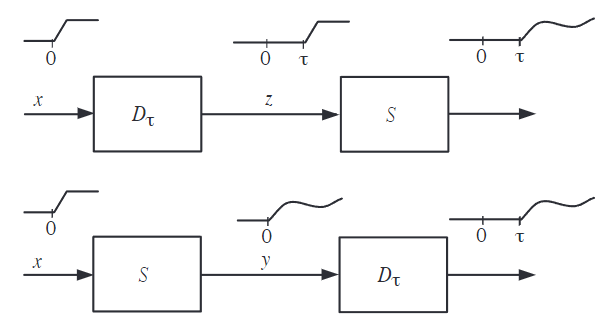
\includegraphics[width=0.7\textwidth]{figs/ln13/time-invariant.png}
        \caption{In time-invariant systems, the system's output from a delayed signal is equal to the delayed system's output of original input.}
    \end{figure}
\end{center}
In another interpretation, we may say that a time-invaraint system $S$ (whose output signal is $y$) receives a delayed input $D_\tau (x)$ and outputs an equivalently delayed output $D_\tau(y)$.
This preservation, or invariance, of shifting in signals is otherwise known as ``shift invariance''.

\section{Linearity of System}
Remember from before that we have defined the linearity of a functino as the intersection of two distinct conditions: superposition and homogeneity:
\[
    \begin{cases}
        (ax)(t) = a(x(t)) \\
        (x_1 + x_2)(t) = x_1(t) + x_2(t)
    \end{cases}
\]
The lineraity of a complex system (systems that map complex-valued functions to complex-valued functions, $S: [\mathbb{C} \rightarrow \mathbb{C}] \rightarrow [\mathbb{C} \rightarrow \mathbb{C}]$) is similarly defined to be the intersection of two conditions:
\[
    \begin{cases}
        (aS)(t) = a(S(t)) \\
        (S_1 + S_2)(t) = S_1(t) + S_2(t)
    \end{cases}
\]

\section{Linearity and Time-Invariance}
Both linearity and time-invariance are realistically fictional properties; that is, they are usually ``ideal properties'' of electronic systems that are not realistically satisfied.
The combination of these useful proeprties provide linear time-invariant systems, which presents the two following simple behaviors:
\begin{enumerate}
    \item Given a sinusoid at the input, the output of an LTI system will be a sinusoid with the same frequency (due to linearity), but possibly with different phase and amplitude (as results of linear transformations, or time-invariance).
    \item Given a weighted sum of sinusoids as an input, the output is a sum of sinusoids with the same frequencies, but possibly different phases and amplitudes.
\end{enumerate}
The most mysterious aspect of the above behavior depiction is perhaps the reason at which phases change. This comes back to a previously introduction of complex exponential expressions for trigonometric functions:
\[
    \forall t \in \mathbb{R}, x(t) = e^{i \omega t} = \cos(\omega t) + i \sin{\omega t}
\]
Under such rule, a delated system's complex exponential expression follows:
\[
    \forall t \in \mathbb{R}, \tau \in \mathbb{R}, x(t - \tau) = e^{i \omega (t - \tau)} = e^{i \omega t} e^{-i \omega \tau}
\]
so the time-invariance of LTI systems allow for delayed inputs, which can lead to the phase changes in a LTI system's output signal from its inputs.

When the output of a system is only a scaled version of the input, the input is called an \textbf{eigenfunction}.
This bodes similarity to eigenvectors in a linear algebra context: while an eigenvector results from a transformation $A$ on a vector $\vec{v}$ that leads to a scaled version of $\vec{v}$, an eigenfunction results from a transformation (system) $S$ that leads to a scaled version of the transformed functions.
Eigenfunctions are convenient in the sense eigenvectors are.

And interestingly, complex exponentials are eignefunctions of LTI systems.
Provided an LTI system,
\[
    \forall t, \tau \in \mathbb{R}, y(t - \tau) = e^{-i \omega \tau} y(t)
\]
At $t = 0$, we see:
\[
    \forall \tau \in \mathbb{R}, y(-\tau) = e^{-i \omega \tau} y(0)
\]
At where $t = -\tau$, $y(t) = e^{i \omega t} y(0)$.
With this transformation $t = -\tau$, we discover that $y(t)$ is an eigenfunction of $e^{i \omega t}$ scaled by $y(0)$, which doesn't depend on time.
Still, we can further discover that this function $y(0)$ does depend on $\omega$ in general, as it is the output evaluated at timestep $0$ provided some input $e^{i \omega t}$.
\[
    \forall \omega \in \mathbb{R}, H(\omega) = y(0) = (S(x))(0), \text{where} \forall t \in \mathbb{R}, x(t) = e^{i \omega t}
\]
Substituting this back to the first expression of this paragraph:
\[
    y(t) = H(\omega) e^{i \omega t}
\]
when the input is $e^{i \omega t}$ and $H(\omega)$ is a function of $\omega \in \mathbb{R}$ (the frequency of the input complex exponential).
Therefore, outside of the argument of our output signal $t$, another moving part to the output of $y(t)$ becomes the frequency of our input signal: $\omega$.
Following such logic, we define for every LTI system a ``frequency response'':
\begin{ln-define}{Frequency Response}{}
    The function $H: \mathbb{R} \rightarrow \mathbb{C}$ is called the frequency response, which defines the response of any LTI system to a complex exponential input at some given frequency, and gives the scaling factor of the system's eigenfunction.
\end{ln-define}

\newpage
\chapter{Frequency Response and Fourier Series}

\section{Finding and Using Frequency Response}
\subsection{Introduction}
To summarize the ending of our previous chapter, for an LTI system, if the input signal is a complex exponential signal $x \in [\mathbb{R} \rightarrow \mathbb{C}]$ such that:
\[
    \forall t \in \mathbb{R}, kx(t) = e^{i \omega t} = \cos(\omega t) + i \sin (\omega t)
\]
then the output of our system $S$ can be written as:
\[
    \forall t \in \mathbb{R}, y(t) = H(\omega) e^{i \omega t}
\]
where $H(\omega)$ is a property of the system we call the frequency response at input frequency $\omega$.

\begin{ln-example}{Frequency Response of the Delay System}{}
    The frequency response of a delay system $S = D_\tau$ for some $\tau \in \mathbb{R}$ is an LTI system, and perhaps the simplest prototype of an LTI system.
    Suppose the input to the delay system is the compelx exponential $x$ given by:
    \[
        \forall t in \mathbb{R}, x(t) = e^{i \omega t}
    \]
    Then the output of the system, $y$, satisfies:
    \[
        \forall t \in \mathbb{R}, y(t) = e^{i \omega (t - \tau)} = e^{-i \omega \tau} e^{i \omega t}
    \]
    And the frequency response of our system output becomes (by matching the definition of frequency response):
    \[
        H(\omega) = e^{-i \omega \tau}
    \]
\end{ln-example}
\begin{ln-example}{Frequency Response of Discrete-time Delay System}{}
    The discrete-time version of a delay system can also becalled the discrete-time $M$-delay system $S = D_M$, where the output of such system is defined as:
    \[
        \forall n \in \mathbb{Z}, y(n) = x(n - M)
    \]
    In such case, we find that the output of such system is:
    \[
        \forall t \in \mathbb{R}, y(t) = e^{i \omega (t - M)} = e^{-i \omega M} e^{i \omega t}
    \]
    where the frequency response of the system is similarly defined as the continuous-time delay system as:
    \[
        H(\omega) = e^{-i \omega M}
    \]
\end{ln-example}

Let us look at another example of solving for frequency responses:
\begin{ln-example}{Frequency Response of Moving Average System}
    Consider the following discrete-time system:
    \[
        \forall n \in \mathbb{Z}, y(n) = \frac{x(n) + x(n - 1)}{2}
    \]
    Then we may observe that when the input for timestep $n$ is $e^{i \omega n}$, the system provides an output:
    \[
        y(n) = \frac{e^{i \omega n} + e^{i \omega (n - 1)}}{2} = \frac{1 + e^{-i \omega}}{2} e^{i \omega n}
    \]
    providing that:
    \[
        H(\omega) = \frac{1 + e^{-i \omega}}{2}
    \]
\end{ln-example}

% TODO: no one has taught about differential equations yet, so they may not handle this? We will write as if students know about these equations now
\subsection{Linear Difference and Differential Equations}
Occasionally, discrete-time systems with input $x$ and output $y$ can be expressed in linear difference equations as exhibited in the previous example.
Here, we provide a shortcut for finding the frequency response of discrete-time systems described with linear difference equations:
\begin{ln-theorem}{Frequency Response of Discrete-time Systems}{}
    For systems described by the lniear difference equation of the form:
    \[
        \forall n \in \mathbb{Z}, \sum_{k = 0}^N a_k y(n - k) = \sum_{i = 0}^M b_k x(n - k)
    \]
    Assuming an input signal of $x(n) = e^{i \omega n}$ and an output signal of $y(n) = H(\omega) e^{i \omega n}$, we obtain the following form of the above difference equation:
    \[
        \forall n \in \mathbb{Z}, \sum_{k = 0}^N a_k H(\omega) e^{i \omega (n - k)} = \sum_{i = 0}^M b_k e^{i \omega (n - k)}
    \]
    which provides that
    \[
        \forall \omega \in \mathbb{R}, H(\omega) = \frac{\sum_{k = 0}^M b_k e^{-i \omega k}}{\sum_{k = 0}^M a_k e^{-i \omega k}}
    \]
\end{ln-theorem}

Then, similarly, for any linear differential equations of the form:
\begin{ln-theorem}{Frequency Response of Continuous-time Systems}{}
    \[
        \forall t \in \mathbb{R}, a_0 y(t) + \sum_{k=1}^N a_k \frac{{\rm d}^k y}{{\rm d} t^k} (t) = b_0 x(t) + \sum_{k=1}^M b_k \frac{{\rm d}^k x}{{\rm d} t^k} (t)
    \]
    With the input signal $x(n) = e^{i \omega n}$ and an output signal $y(n) = H(\omega) e^{i \omega n}$, we may first recognize that:
    \[
        \frac{\rm{d}^k}{\rm{d} t^k} e^{i \omega t} = {(i \omega)}^k e^{i \omega t}
    \]
    we may find that the above linear differential equation can be presented as:
    \[
        \sum_{k = 0}^N a_k H(\omega) {(i \omega)}^k e^{i \omega t} = \sum_{k = 0}^M b_k H(\omega) {(i \omega)}^k e^{i \omega t}
    \]
    which leads to the frequency response formula:
    \[
        \forall \omega \in \mathbb{R}, H(\omega) = \frac{\sum_{k = 0}^M b_k {i \omega}^k}{\sum_{k = 0}^M a_k {i \omega}^k}
    \]
\end{ln-theorem}

\subsection{Frequency Response with Complex Exponentials}
Recall that real-valued sinusoidal signals can be written as a combination of exponential signals; for example:
\[
    \cos(\omega t) = \frac{e^{i \omega t} + e^{-i \omega t}}{2}
\]
Which leads to an output signal of:
\[
    y(t) = \frac{H(\omega) e^{i \omega t} + H(-\omega) e^{-i \omega t}}{2}
\]
However, most LTI systems are not capable of producing complex-valued outputs provided real inputs.
Assuming that $y(t)$, the output signal, is real, we would need that $H(\omega) e^{i \omega t} + H(-\omega) e^{-i \omega t}$ must also be real.
For the imaginary aspects of these two terms to cancel,
\[
    Im{H(\omega) e^{i \omega t}} + Im{H(-\omega) e^{-i \omega t}} = 0
\]
Note that,
\[
    H(\omega) e^{i \omega t} = H(\omega) (\cos(\omega t) + i \sin(\omega t))
\]
Therefore,
\[
    Im(H(\omega) e^{i \omega t}) = Re{H(\omega)} \sin(\omega t) + Im{H(\omega)} \cos(\omega t)
\]
And, applying this fact on both sides of the prior equation (about cancelling imaginary parts) leads us to the equation:
\[
    Re{H(\omega)} \sin(\omega t) + Im{H(\omega)} \cos(\omega t) = -Re{H(-\omega)} \sin(-\omega t) - Im{H(-\omega)} \cos(-\omega t)
\]
Leading to the conclusion that:
\[
    Im{H(\omega) e^{i \omega t}} = -Im{H(-\omega) e^{-i \omega t}}
\]
This conclusion is otherwise known as conjugate summetry.

Based on conjugate symmetry, we further claim that when the input of our LTI system is $x(t) = \cos(\omega t)$, the output of the system is:
\[
    \forall t \in \mathbb{R}, y(t) = Re{H(\omega) e^{i \omega t}}
\]
Note that by the polar expression,
\[
    H(\omega) = |H(\omega)| e^{i \angle H(\omega)}
\]
And therefore, upon some mathematical derivation using Euler's Law, we find that:
\[
    \forall t \in \mathbb{R}, y(t) = |H(\omega)| \cos(\omega t + \angle H(\omega))
\]
which presents the gain $|H(\omega)|$ (magnitude response), phase shift $\angle H(\omega)$ (phase response) of a sinusoidal input with frequency $\omega$.

\section{Frequency Response with Fourier Series}
\subsection{Fourier Series with Complex Exponentials}
Hi

\subsection{Solving Coefficients of Fourier Series}
Hello

\subsection{Frequency Response and Fourier Series}
Hello

\section{Frequency Response of Composite Systems}
\subsection{Cascade Connection}
Hello

\subsection{Feedback Connection}
Hello

\newpage
\chapter{Introduction to Filtering}

\section{Convolution}
\subsection{Convolution Sum and Convolution Integral}
Hello

\subsection{Impulses}
Hello

\subsection{Weighted Sum of Delta Functions}
Hello

\section{Impulse Response}
\subsection{Impulse Response and Convolution}
Hello

\subsection{Impulse Response and Frequency Response}
Hello

\newpage
\chapter{Impulse Resopnse Filters}
Hello

\part{Sampling and Fourier Transform}
\chapter{The Four Fourier Transforms, Part I}

\section*{Notations}
Hello

\section{Continuous-Time Fourier Series}
Hello

\section{Discrete Fourier Transform}
Hello

\newpage
\chapter{The Four Fourier Transforms, Part II}

\section{Discrete-Time Fourier Transform}
Hello

\section{Continuous-Time Fourier Transform}
Hello

\newpage
\chapter{Fourier Transform vs. Fourier Series}
Hello
\newpage
\chapter{Sampling and Reconstruction}

\section{Sampling}
\subsection{Sampling and Aliasing}
Hello

\subsection{Perceived Pitch Experiment}
Hello

\subsection{Aliasing Ambiguities}
Hello

\section{Reconstruction}
\subsection{Survey and Introduction}
Hello

\subsection{Mathematical Assumptions of Reconstruction}
Hello

\newpage
\chapter{The Nyquist-Shannon Sampling Theorem}
Hello

\end{document}
